\section{Applying Transport Classification Concept}

Contaminant entry from the subsurface into the a building may be dominated by advection or diffusion and which it is dramatically changes how a structure is expected to respond to change in building pressurization.
For diffusion dominated sites, contaminant entry rates will be relatively decoupled from building pressurization, except in the limit where the building is sufficiently pressurized relative to the subsurface that the diffusion pathway is effectively cut off.
This has implications for a wide variety of VI investigation strategies, but is perhaps most relevant for attempting to use CPM and choosing the relevant ITS parameters for study.\par

\subsection{The Controlled Pressure Method}

The idea of CPM is to control internal building pressurization, e.g. by using some fans or blowers to induce a higher or lower than ambient pressure in the structure.
The normal expectation is that this will in turn control the contaminant entry rate.
The underlying assumption in application of this method is that contaminant entry into a building is largely advective in nature.
Because the effect of minor pressure fluctuations on diffusion coefficients is negligible, the only effect that such a building pressure variation can have is in adjusting the advective flow that either promotes or impedes the diffusive flux.
But as the preceding Péclet number analysis has already shown, most cases are quite far towards the limit of diffusion control, and so small changes in advective entry rates will have minor effects on diffusive entry rates.
Thus at "diffusion-controlled sites" the CPM method will not be as effective.\par

Figure \ref{fig:cpm_adv_diff} further illustrates this point.
Reconsidering the case of the ASU house analysis already discussed in Chapter \ref{chp:preferential_pathways}, during the period when the land drain preferential pathway was open, CPM dramatically increased indoor contaminant concentrations compared to the when the CPM system was inactive.
However, after the closing of the land drain preferential pathway, CPM did not have any significant effect on measured indoor contaminant concentrations.
From the modeling of this situation, it was deduced that the presence of the land drain preferential pathway made advection the dominant entry mechanism of contaminant vapors into the building.
Once that pathway was closed, the influence of a significant depressurization of the building was rather muted, because the basic diffusive entry pathway was largely unaffected.\par

\begin{figure}[htb!]
  \centering
  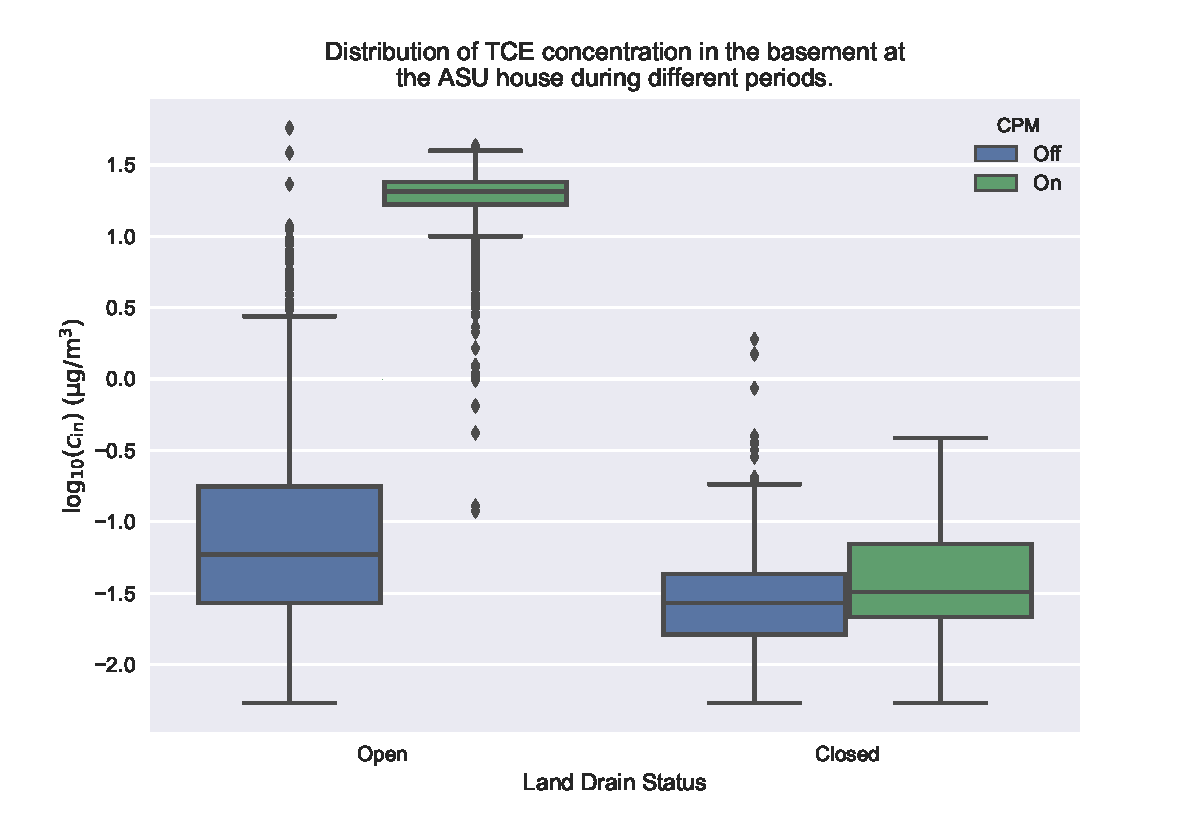
\includegraphics[width=0.75\textwidth]{asu_boxplot_concentration.pdf}
  \caption[Boxplot showing the log-10 transformed TCE concentrations measured at the ASU house as a function of whether the preferential pathway was open or closed.]{Boxplot showing the log-10 transformed TCE concentrations measured at the ASU house as a function of whether the preferential pathway was open or closed. The measured contaminant concentrations obtained during the reduced pressure CPM and "natural" vapor intrusion periods are considered separately. The box signifies the interquartile range (IQR) of values, with the central line representing the median value, and the top and bottom of the box are the \nth{25} and \nth{75} percentiles. The whiskers extend to 1.5 times the IQR. Markers indicate outlier data points that fall outside the whiskers.}
  \label{fig:cpm_adv_diff}
\end{figure}

The above results warn that depressurization of a structure using CPM might not lead to the expected result of a significant increase in entry rate of contaminant.
Proponents of the technique argue that the method can offer a "worst possible case" result for a particular building, because the employed depressurization will be greater than anything that would naturally be encountered in the structure.
This thinking is clearly influenced by a conceptual model that views advective entry as a dominant entry mode.
The logic that such depressurization will offer a "worst possible case" result is actually not flawed, because enhancing contaminant entry rate is a real consequence of the depressurization.
What will not be as apparent in the results from a diffusive entry limited case is that there is any relationship between the degree of depressurization and entry rate (and thus, indoor air concentration); there is a good chance that any small increase in concentration would be lost in the normal "noise" of such concentration measurements.
The true value of the CPM can come in cases in which there is an obvious and large increase in entry rate with the degree of depressurization; in those cases, there will be a clear indication of either a permeable soil or the existence of a preferential pathway that can support advective entry as the dominant mode of contaminant entry.\par

There is an additional consideration that should not be overlooked when conducting a CPM investigation of VI.
CPM not only affects the contaminant vapor entry rate into a building, but can also have an impact on air exchange rates within the building being tested.
Figure \ref{fig:asu_cpm_ae} shows the effect that CPM had on air exchange rates at the ASU house, where they increased significantly during the testing period.
The effect of this is that contaminant expulsion from the house is increased during the testing period, which decreases the indoor contaminant concentration for a given contaminant entry rate.
This is a concern voiced in \cite{holton_long-term_2015}\cite{holton_long-term_2015} an evaluation of the CPM results at the ASU house, and suggested that a tracer-gas test to measure air exchange rate should be conducted during CPM.
This is used to introduce a correction term to account for the elevation of air exchange rate above its "natural" values.
Since CPM is used to determine the worst-case scenario, this correction term should be used to calculate the indoor contaminant concentration with worst-case entry rates, but "natural" air exchange rate values, i.e. $\approx \SI{0.5}{\per\hour}$ instead of the elevated values.
In this case, it is apparent that the measured values of indoor air concentration might have been a factor of 5 or 6 lower than would otherwise have been obtained for the given change in entry rate.
This means that the results in Figure \ref{fig:cpm_adv_diff} might have understated the effect of the entry rate change. \par

\begin{figure}[htb!]
  \centering
  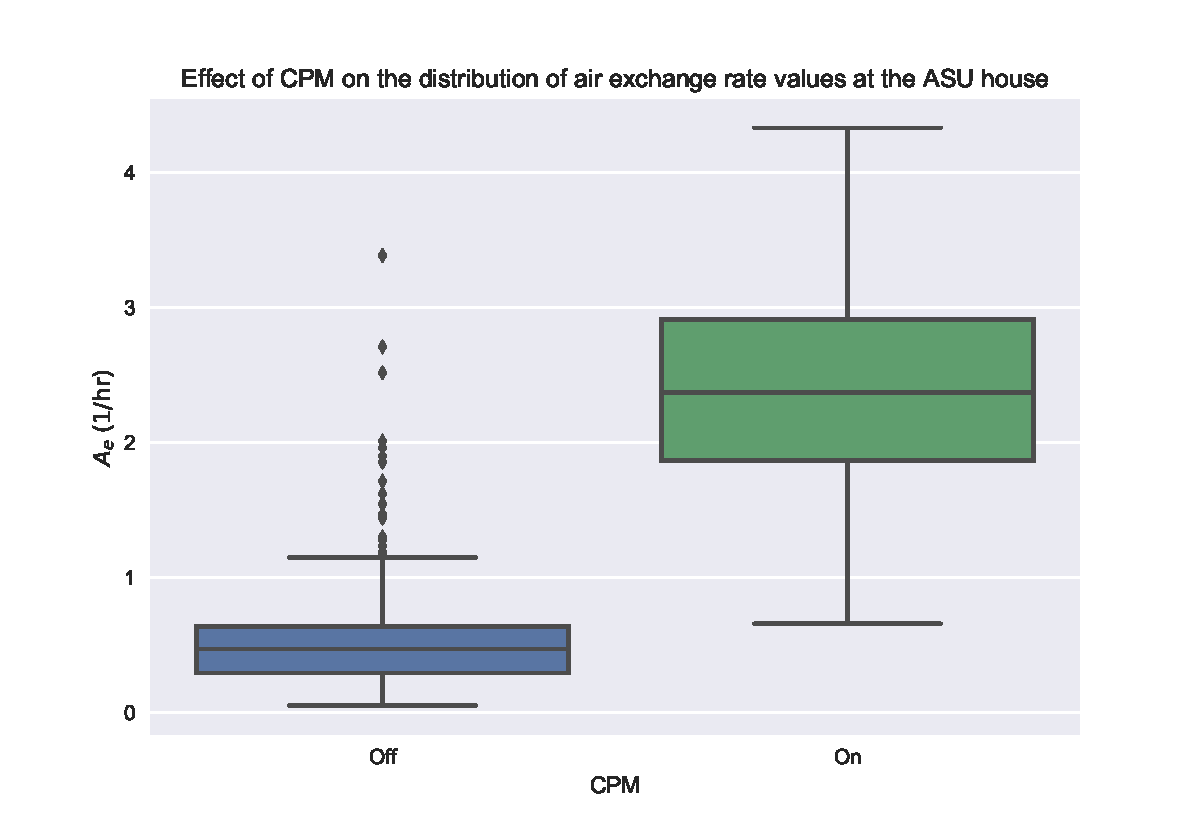
\includegraphics[width=0.75\textwidth]{asu_cpm_ae.pdf}
  \caption{Boxplot showing the distribution of air exchange rate values at the ASU house, considering the effect of CPM.}
  \label{fig:asu_cpm_ae}
\end{figure}

This highlights an issue with CPM at VI sites characterized by diffusive transport.
If the increased depressurization doesn't yield higher contaminant entry rates into the building, but elevates air exchange rate, then indoor contaminant concentration may be artificially lowered, and actually underestimate the VI risk.
This further shows the advisability of using tracer-gas monitoring to measure air exchange rates when using CPM.\par

\subsection{Indicators, Tracers, And Surrogates}

As has been discussed throughout this work, VI can be characterized by great temporal variability in indoor air contaminant concentrations.
These variations can occur on a variety of time-scales, from days to longer seasonal trends, which can require collection of significant amounts of data to fully characterize.
To reduce the resources expended on these efforts, and increase the likelihood of determining the relevant VI risk, it is desirable to employ indicators, tracers, and surrogates (ITS) that can be used to readily predict the periods and conditions when the highest indoor contaminant concentration at a site are likely to manifest.
Which specific ITS are most appropriate for this task, and under which circumstances they are reliably employed has, has yet to be determined.\par

\begin{figure}[htb!]
  \centering
  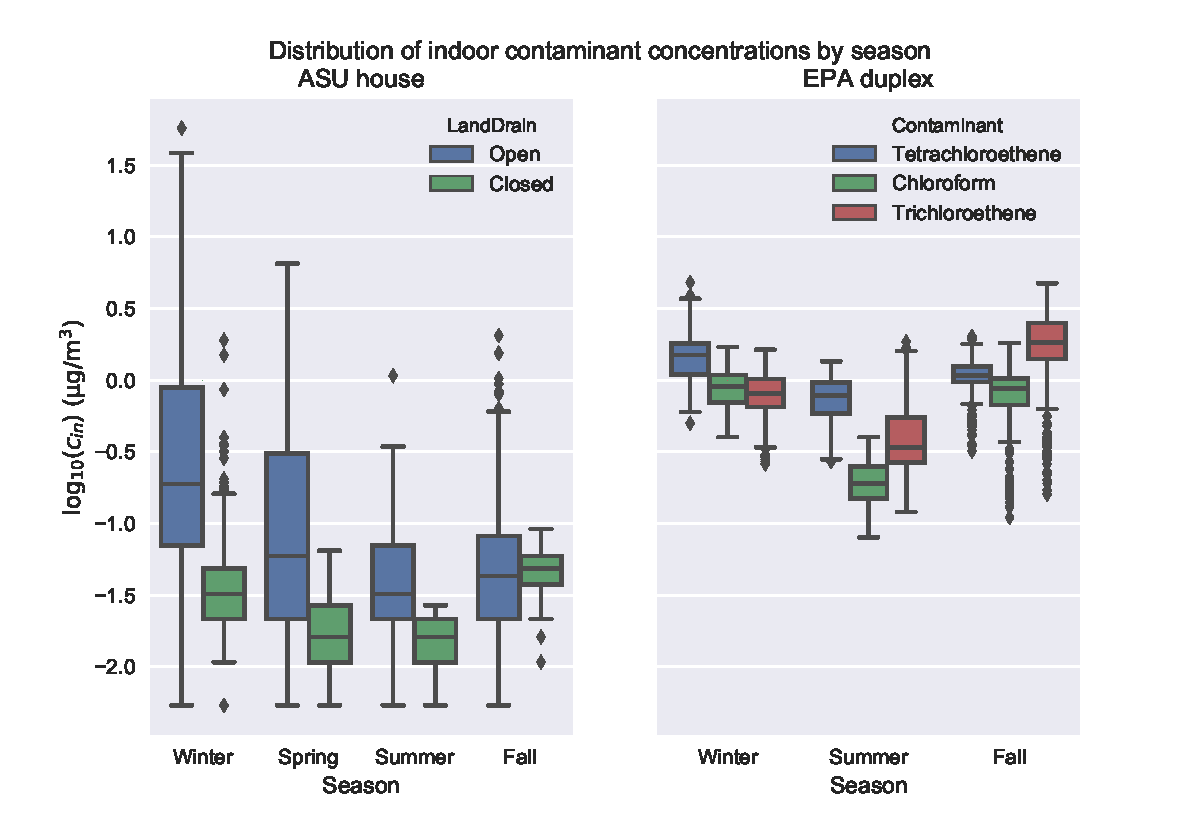
\includegraphics[width=\textwidth]{seasonal_concentration.pdf}
  \caption[Seasonal distribution of indoor contaminant concentration at the ASU house and EPA duplex.]{Seasonal distribution of indoor contaminant concentration at the ASU house and EPA duplex. At the ASU house, the effect of the land drain preferential pathway is considered. At the EPA duplex, the differences in distribution for three different contaminants are considered. Here "winter" includes December to February, with each subsequent season being defined by the subsequent three months.}
  \label{fig:seasonal_concentration}
\end{figure}

Seasonal trends have been to observed to be common at many VI sites, with winter often cited as the period most likely to lead to measurements of elevated indoor contaminant concentrations\cite{burke_estimation_2010,hers_evaluation_2014,miles_temporal_2001,schumacher_fluctuation_2012,steck_indoor_2004}.
This is a trend that partly occurred at the ASU house as well (see Figure \ref{fig:seasonal_concentration}); indoor contaminant concentrations were indeed highest during winter when the land drain preferential pathway was open.
However, this seasonal trend was non-existent after the closing of the land drain.
At the EPA duplex, indoor contaminant concentrations were slightly higher during winter and fall than summer, but only marginally so.\par

\begin{figure}[htb!]
  \centering
  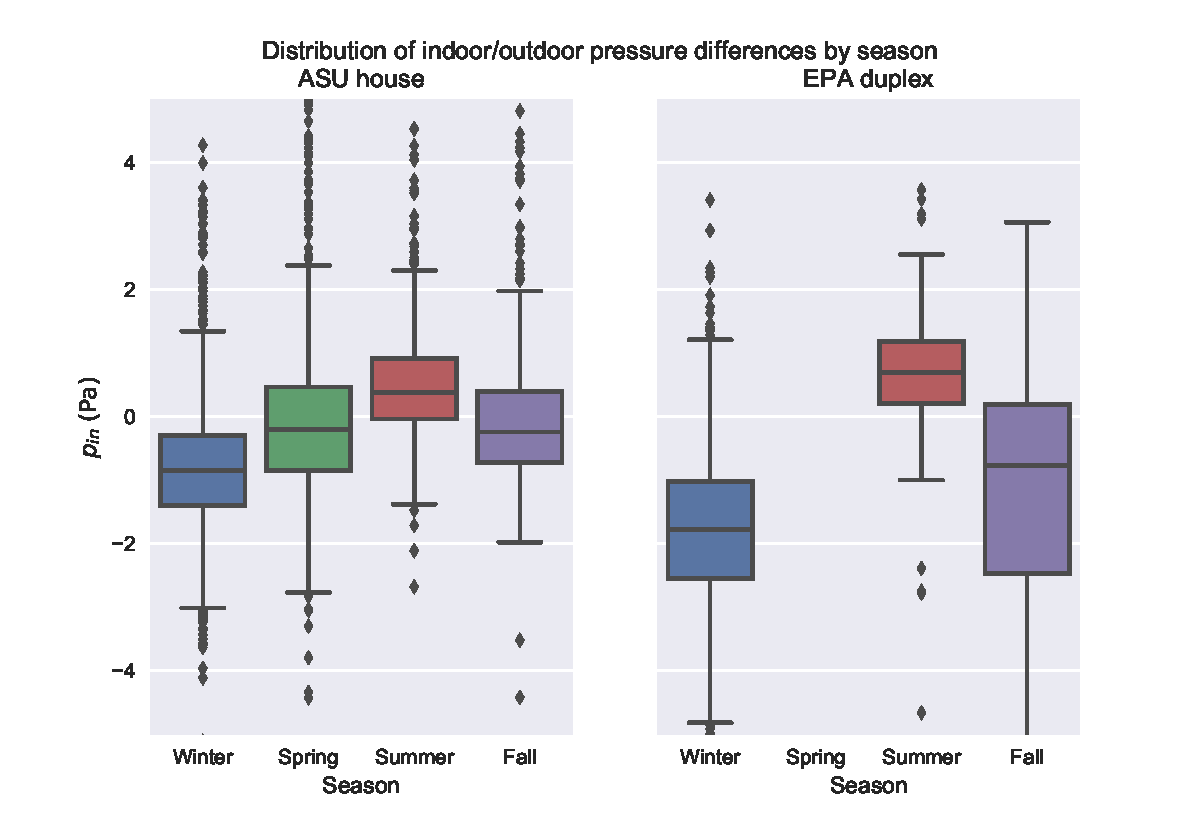
\includegraphics[width=\textwidth]{seasonal_pressure.pdf}
  \caption[Seasonal distribution of indoor contaminant concentration at the ASU house.]{Seasonal distribution of indoor contaminant concentration at the ASU house. A negative value indicates that the building is depressurized relative to ambient.}
  \label{fig:seasonal_pressure}
\end{figure}

The observed seasonal trend at the ASU house when the preferential pathway was open, can be understood by examining the seasonal distribution of indoor/outdoor pressure difference, displayed in Figure \ref{fig:seasonal_pressure}.
Here we see that building depressurization was greatest during winter, and that the house was slightly less depressurized during the shoulder seasons, and it was  usually overpressurized during summer.
Considering this together the fact that with advective entry dominated during the period when the preferential pathway was open, explains why indoor contaminant concentrations are higher during the colder seasons.
The significant degree of depressurization in winter contributed significantly to what was an advectively determined entry rate during that period of time.
The opposite would have been true during summer, when it is likely that the use of air conditioning slightly overpressurized the building.
Conversely, when the preferential pathway was closed off, the entry of contaminant shifted to being diffusion rate controlled, and the variations in internal building pressure had little effect on the entry rate.\par

The EPA duplex exhibited a trend in building pressurization by season that is similar to that observed at the ASU house, i.e. it is more depressurized during colder seasons.
This can help explain why indoor contaminant concentrations were likewise slightly higher during colder seasons.
While the nature of the contaminant entry into the EPA duplex is not as well understood as that at the ASU house, it was shown in Chapter \ref{chp:preferential_pathways} that the association between building pressurization and indoor contaminant concentrations were somewhere between that of the ASU house before and after the closing of the preferential pathway (compare Figures \ref{fig:asu_pressure_dependence} and \ref{fig:indie_pressure_dependence}).
The situation regarding likely entry pathways at the EPA duplex is far more complicated and less well understood than that at the ASU house.

All that can be said at the moment is that while advective contaminant entry may not be dominant at the EPA duplex, it certainly isn't insignificant.\par

These data and analysis demonstrate that for advection entry controlled sites, building pressurization can probably be used as an effective ITS, whereas at a diffusion entry site, it may not be reliable.
The advection entry controlled sites are those built on very permeable soils, or which are influenced by some preferential pathway, which allows advective entry to be the dominant entry pathway.
This by itself may be challenging to determine in advance.
Even if this could be established, to use building pressurization effectively as an ITS, building pressurization values would need to be known, and instrumenting a house to obtain such values is not generally feasible in VI screening studies.
Instead, it would be useful to be able to predict the likely levels of indoor-outdoor pressure difference based on some easier to measure parameters - such as weather conditions.\par
